\documentclass[12pt,reqno]{article}

%%%%%%%%%%%%%%%%%%%% PACKAGES %%%%%%%%%%%%%%%%%%%%

\usepackage[utf8]{inputenc}
\usepackage[all]{xy}
\usepackage[T1]{fontenc}
\usepackage[usenames, dvipsnames]{color}
\usepackage{setspace}
\usepackage{dsfont}
\usepackage{amssymb}
\usepackage{amsthm,bbm}
\usepackage{amscd}
\usepackage{amsfonts}
\usepackage{stmaryrd}
\usepackage{amsmath}
\usepackage{graphicx}
\usepackage{multicol}
\usepackage{xspace}
\usepackage{extarrows}
\usepackage{color}
\usepackage [english]{babel}
\usepackage [autostyle, english = american]{csquotes}
\usepackage[colorlinks, linktocpage, citecolor = red, linkcolor = blue]{hyperref}
\usepackage{fullpage}
\usepackage{color}
\usepackage{euler}

%%%%%%%%%%%%%%%%%%%% INITIALIZATION %%%%%%%%%%%%%%%%%%%%

\MakeOuterQuote{"}
\graphicspath{ {./} }
\setlength{\parskip}{\baselineskip}
\setlength{\parindent}{0pt}

%%%%%%%%%%%%%%%%%%%% COMMANDS %%%%%%%%%%%%%%%%%%%%

\newcommand{\range}{\mathrm{range\,}}
\newcommand{\nul}{\mathrm{null\,}}
\newcommand{\spn}{\mathrm{span\,}}
\newcommand{\card}{\mathrm{cardinality}}
\newcommand{\R}{\mathbb{R}}
\newcommand{\C}{\mathbb{C}}
\newcommand{\F}{\mathbb{F}}
\newcommand{\Z}{\mathbb{Z}}
\newcommand{\bd}{\mathrm{bd\,}}
\newcommand{\divline}{\hrule\vspace{12pt}\noindent}
\newcommand{\sgn}{\mathrm{sgn}}

%%%%%%%%%%%%%%%%%%%% ENVIRONMENTS %%%%%%%%%%%%%%%%%%%%

\theoremstyle{definition}
\newtheorem{problem}{Problem}

%%%%%%%%%%%%%%%%%%%% TITLE-PAGE %%%%%%%%%%%%%%%%%%%%

\title{MATH 1530 Problem Set 1}
\author{Collaborated with Esmé and Kazuya}
\date{February 2023}

%%%%%%%%%%%%%%%%%%%% DOCUMENT %%%%%%%%%%%%%%%%%%%%

\begin{document}
\maketitle

%%%%%%%%%%%%%%%%%%%% PROBLEM 1 %%%%%%%%%%%%%%%%%%%%

\begin{problem} 
Please read the article \href{https://www.scientificamerican.com/article/the-secret-to-raising-smart-kids1/}{The secret to raising smart kids} in Scientific American.

Do you think you have a growth mindset when it comes to learning math? Do you think learners of mathematics usually have a growth mindset? What can you do to develop a growth mindset?
\end{problem}

I think I have a growth mindset in the sense that I believe mathematics is a skill that (like most other things) can be learned and improved upon with time and continued effort. I am fairly patient and don't give up when a question confuses me. I think that you sort of have to have a growth mindset to make it far in mathematics because at the forefront of the field, there are myriad problems that have stumped everyone. It is a mathematician's job to solve these problems, and so you inherently have to be willing to accept hitting dead-ends and stay determined. Believing in myself and practicing are two ways that I think I can keep having a growth mindset.

\newpage

%%%%%%%%%%%%%%%%%%%% PROBLEM 2 %%%%%%%%%%%%%%%%%%%%

\begin{problem}
    Prove that $5n+3$ and $7n+4$ are relatively prime for all integers $n$.
\end{problem}

\begin{proof}
    To prove that $5n+3$ and $7n+4$ are relatively prime, we will prove that 
    \begin{align*}
        gcd(5n + 3, 7n + 4) &= 1 & \text{(definition of relative primeness)}
    \end{align*}
    $gcd(5n + 3, 7n + 4)$ must be the smallest positive integer that can be expressed as the linear combination $s(5n+3) + t(7n+4)$ (Gallian, Theorem 0.2). By fixing $s$ and $t$ to $7$ and $-5$ respectively, we have
    \begin{align*}
        7(5n+3) - 5(7n+4) = 1
    \end{align*}
    $1$ is the smallest positive integer, thus we have proven that $gcd(5n + 3, 7n + 4) = 1$.
\end{proof}

\newpage

%%%%%%%%%%%%%%%%%%%% PROBLEM 3 %%%%%%%%%%%%%%%%%%%%

\begin{problem} 
Prove that $a^2-1$ is divisible by 8 for all odd integers $a\geq 3$.
\end{problem}

\begin{proof}
We will use induction.

Base case: Let $n = 3$. We have that $8\ |\ 3^2 - 1$.

Induction Step: Let $n \geq 3$ be an integer. Suppose that for all odd integers within the range $3 \leq a \leq n$, we have that $8\ |\ a^2 - 1$.

We will now prove that $8\ |\ (n + 2)^2 - 1$.
\begin{align*}
    (n + 2)^2 - 1 &= n^2 + 4n + 4 - 1\\
    &= (n^2 - 1) + 4(n + 1)
\end{align*}
From the inductive hypothesis, we have that $8\ |\ n^2 - 1$. In other words, there exists some integer $b$ such that $n^2 - 1 = 8b$. Additionally, $n + 1$ will always be an even integer, meaning there exists some integer $c$ such that $n+1 = 2c$. Thus, $4(n+1) = 8c$. Therefore, since $(n^2 - 1) + 4(n + 1) = 8(b + c)$, we can conclude that $8\ |\ (n+2)^2 - 1$.
\end{proof}

\newpage

%%%%%%%%%%%%%%%%%%%% PROBLEM 4 %%%%%%%%%%%%%%%%%%%%

\begin{problem} 
If $a,b \in \mathbb{Z}$, define $a \sim b$ if $ab \geq 0$. Is $\sim$ an equivalence relation on $\mathbb{Z}$?
\end{problem}

\begin{proof}
    Let $a,b,c\in\Z$ such that $a = -1$, $b=0$, $c=1$.

    It follows that $a \sim b$ and $b\sim c$, since $-1 \cdot 0 \geq 0$ and $1\cdot 0 \geq 0$. By the transitive property, we have that $a\sim c$. However, $a\nsim c$ because $-1\cdot 1 \ngeq 0$. Thus, we have reached a contradiction, proving that $\sim$ is not an equivalence relation on $\Z$. 
\end{proof}

\newpage

%%%%%%%%%%%%%%%%%%%% PROBLEM 5 %%%%%%%%%%%%%%%%%%%%

\begin{problem} 
For $a,b \in \mathbb{R}$, define $a \sim b$ if $a - b$ is an integer. Show that $\sim$ is an equivalence relation on $\mathbb{R}$. Describe the equivalence classes of $\sim$. Bonus: can you draw a picture of the set of equivalence classes?
\end{problem}

\begin{proof}
    To prove that $\sim$ is an equivalence relation on $\R$, we will prove that it is reflexive, symmetric, and transitive.
    
    Reflexive: Let $a\in\R$. $a-a=0\in\Z$, therefore $a\sim a$.

    Symmetric: Let $a,b\in\R$. If $a\sim b$, we have that $a-b = c \in\Z$. Thus, $b-a=-c\in\Z$. Therefore, $a\sim b$ implies $b\sim a$.

    Transitive: Let $a,b,c\in\R$. If $a\sim b$ and $b\sim c$, we have that $a-b=d\in\Z$ and $b-c=e\in\Z$. Thus, $a-c=d+e\in\Z$. Therefore, we have that $a\sim b$ and $b\sim c$ implies that $a\sim c$.
\end{proof}

The equivalence classes of $\sim$ can be defined by $\left[a\right] = \{a + k\ |\ k\in\Z\}$. Using this definition, the equivalence classes can be visualized on a coordinate plane with the brown line on the $x$ axis representing the choice of $a$ and each diagonal line depicting a representative set:

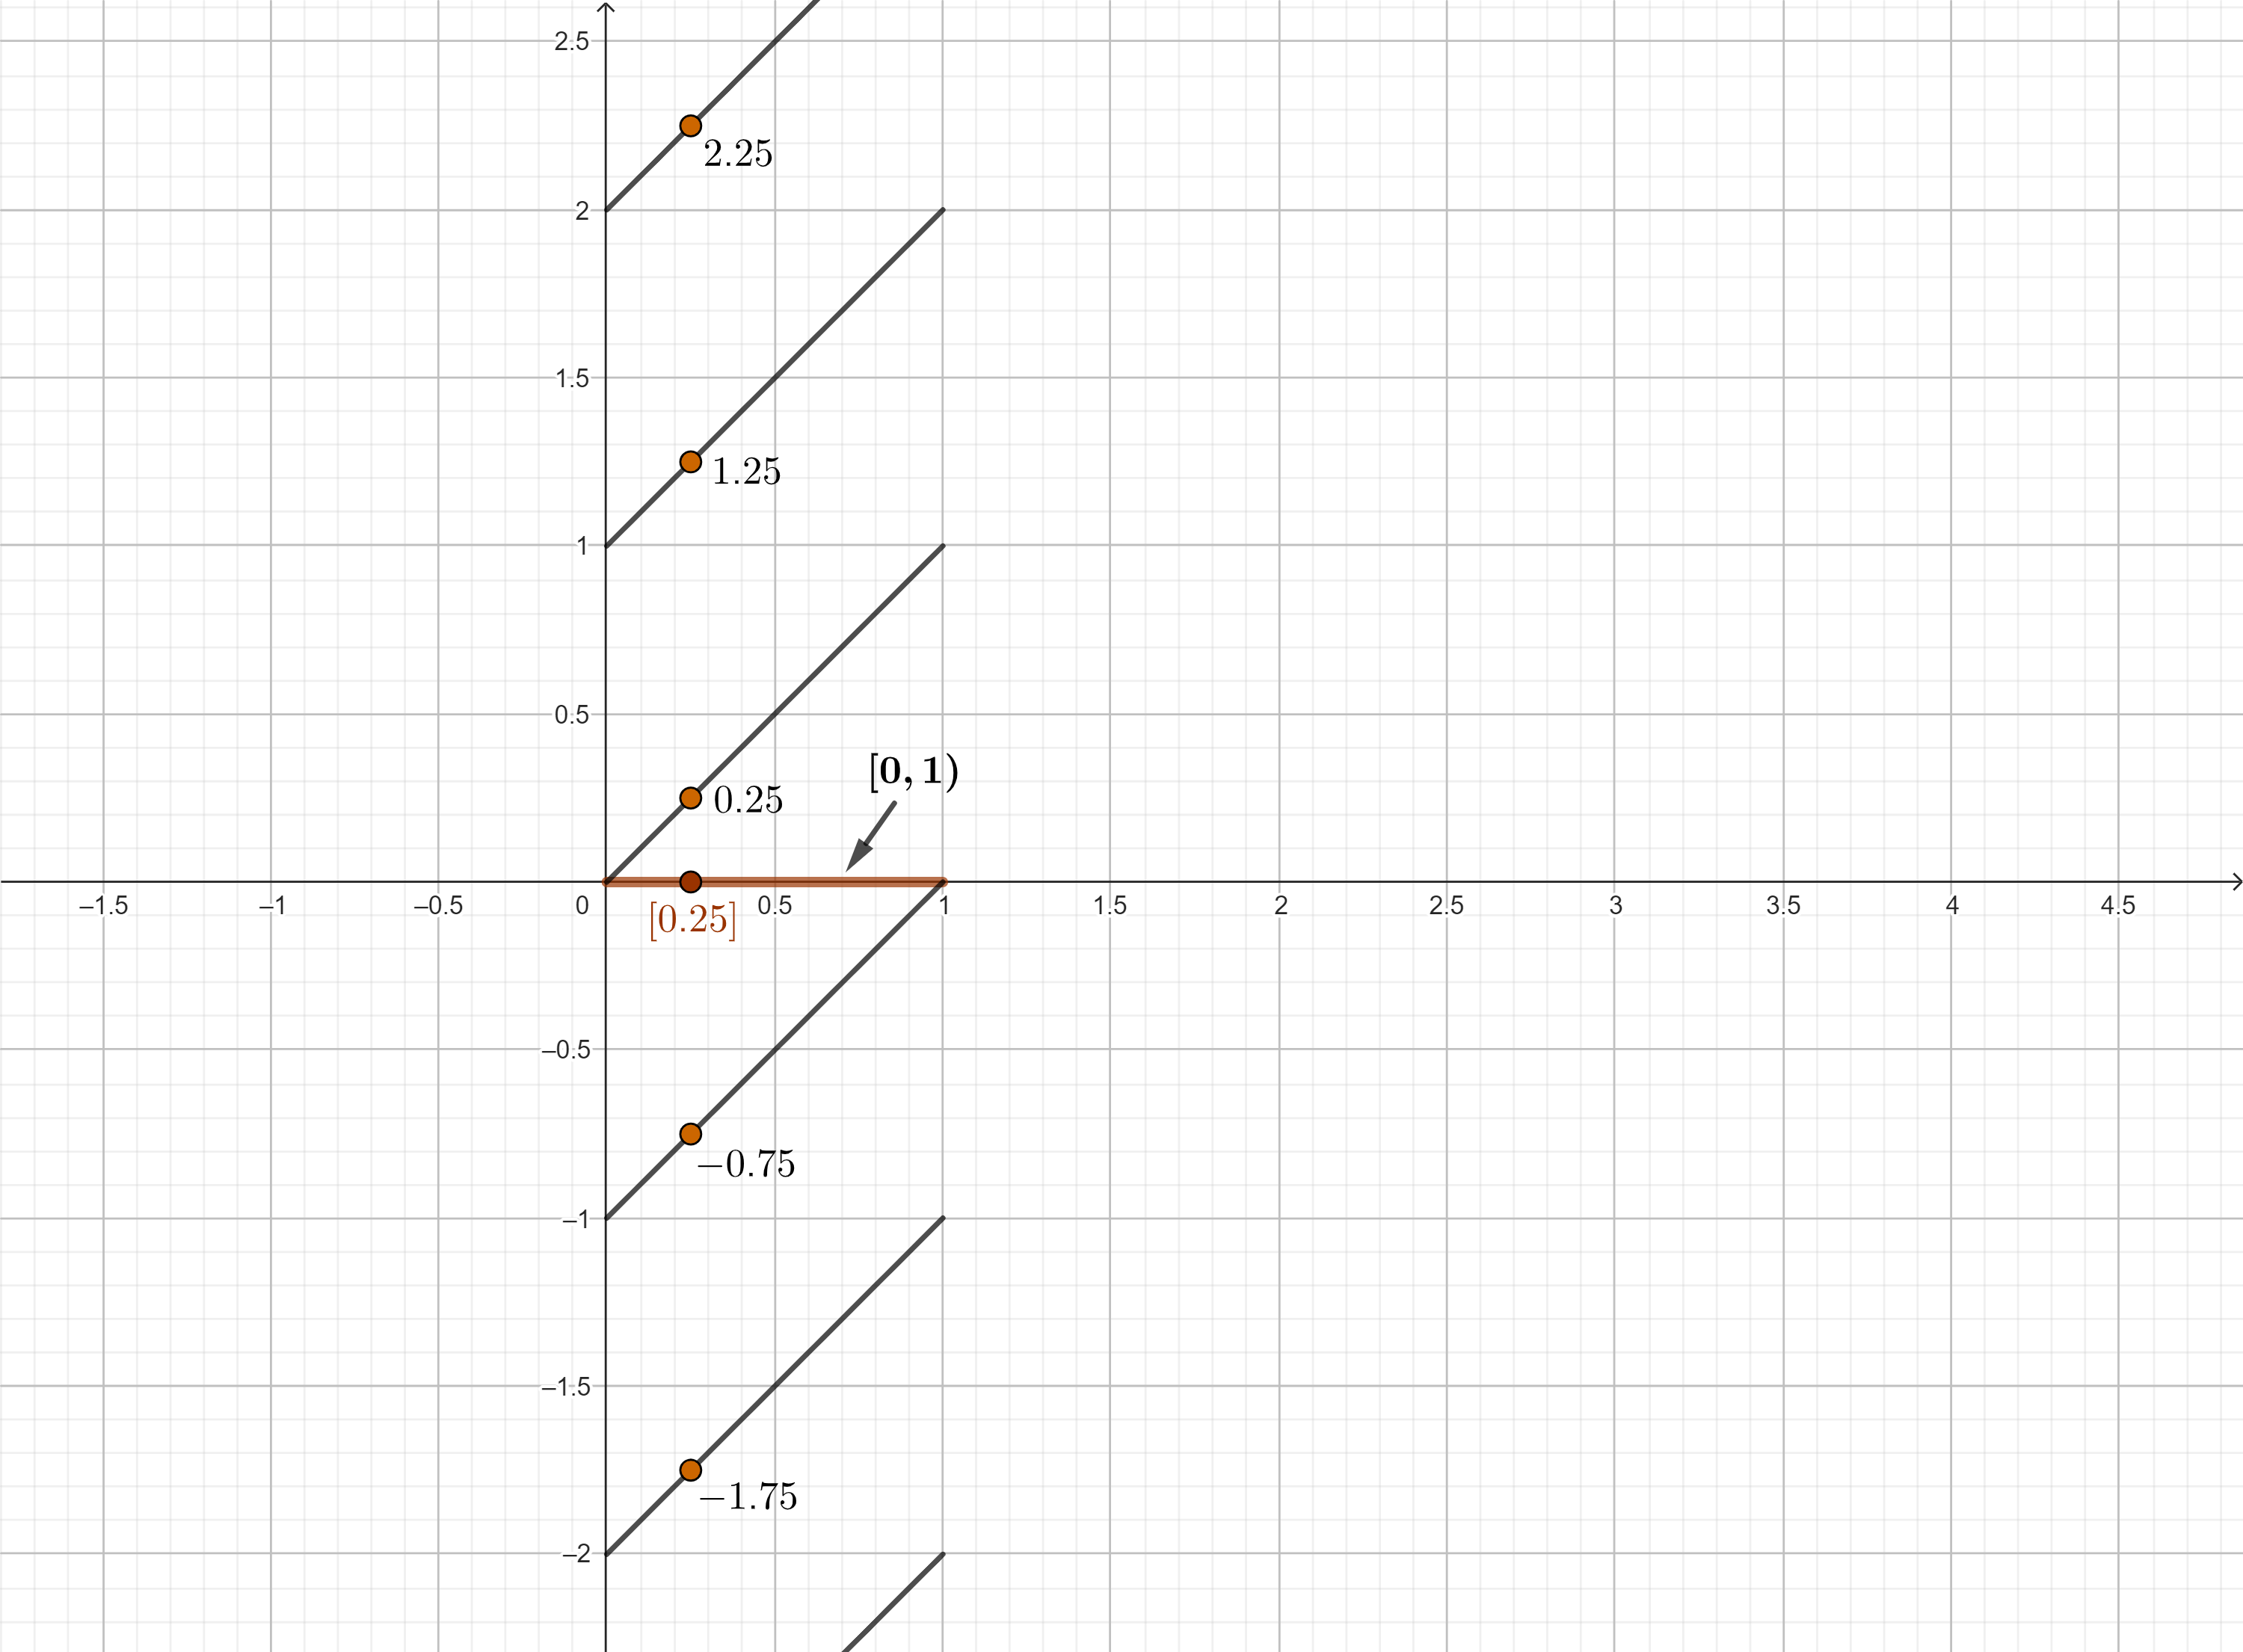
\includegraphics[scale=2.35]{MATH 1530 P1.png}

\end{document}